
In the following chapter will be discussed shortly two attitude controller designs that are based on previous work \cite{PrevPro}. The two controllers calculate a torque demand that has to be produced from the motors. The first controller is based on the linearized model \eqref{eq:lele}, and thus is characterized as linear state feedback control, while the second one is based on the non-linear dynamics \eqref{eq:seom} creating a sliding manifold, a hyperplane, such that when the states are on the manifold, will converge to the desired reference. The non-linear controller is called Sliding Mode Control (SMC).\nomenclature[A]{\textbf{SMC}}{Sliding Mode Control}

\section{Linear controller} \label{sec:LC}

Since the norm of $ \vec{ {\bar{\omega}}} $ is known and equal to the orbital angular velocity ($\approx 0.0011$) comparing this value to $\frac{1}{2}$,becomes small, thus \eqref{eq:lele} can be simplified to 
\begin{flalign}
	\begin{bmatrix}
		\vec{ \dot {\tilde{q}}(t) } \\
		\vec{ \dot {\tilde{\omega}}(t) }
	\end{bmatrix} 	
	= 
	\begin{bmatrix}
		\underline{ 0}_{(3\times3)} &	\frac{1}{2} \underline{\vec 1}_{(3\times3)} \\
		\underline{ 0}_{(3\times3)} &	\underline{ 0}_{(3\times3)}
	\end{bmatrix} 
	\begin{bmatrix}
		\vec{  {\tilde{q}}(t) } \\
		{  {\tilde{\vec \omega}}(t) }
	\end{bmatrix} 	
	-
	\begin{bmatrix}
		\underline{\vec 0}_{(3\times3)} \\
		{\underline I_{s}^{-1}}
	\end{bmatrix} 	
	\vec {\tilde N_{ctrl}}
	\label{eq:lelele}
\end{flalign}
Three equal subsystems can be derived from \eqref{eq:lelele} as
\begin{flalign}
	\begin{bmatrix}
		\dot { \tilde {q_{i}}} \\
		\dot { \tilde { \omega_{i}}}
	\end{bmatrix} 	
	= 
	\begin{bmatrix}
		0&	\frac{1}{2}  \\
		0 &	 0
	\end{bmatrix} 
	\begin{bmatrix}
		\tilde{q_{i}}(t)  \\
		\tilde{\omega_{i}}(t) 
	\end{bmatrix} 	
	-
	\begin{bmatrix}
		0 \\
		I_{i,s}^{-1}
	\end{bmatrix} 	
	\tilde{N_{i}}
	\label{eq:subsys}
\end{flalign}
with $i = 1, 2, 3 $. The control torque was defined by the state feedback law as 
\begin{flalign}
	N_{i}	
	= 
	-
	\begin{bmatrix}
		k_{1} &	k_{2} 	
	\end{bmatrix} 
	\begin{bmatrix}
		\tilde{q_{i}}(t)  \\
		\tilde{\omega_{i}}(t) 
	\end{bmatrix} 	
	\label{eq:inputtorque}
\end{flalign}
leading to a second order closed loop system calculated as $det(s\underline{I} - (\underline{A} - \underline{BK}) )$. Identifying  this with a general second order equation $s^{2}+2\zeta\omega_{n}s+\omega_{n}^{2}$, with $\zeta$ be the dumping factor which was chosen to be equal to 1 leading to an over dumped response and $\omega_{n}$  the natural frequency $\omega_{n} =  \frac{2\pi}{60/0.35} $ with 60 be the value of the chosen rise time, the controller gains was derived as

\begin{flalign*}
	k_{1} = -2 I_{i,s} \omega_{n}^{2} 
	\label{eq:gainsl22}
\end{flalign*}
\begin{flalign*}
	k_{2} = -2\zeta I_{i,s} \omega_{n}^{2} 
	\label{eq:gainsl223}
\end{flalign*}
which give stability for the all values of $ \vec{ {\bar{\omega}}} $. 
\section{Sliding mode control} \label{sec:SM}

As described previously the sliding mode control scheme belongs to the class of non-linear control designs and is more robust compared to the linear, when disturbances are present. The objective of the SMC is the design, from a geometrical point of view, of a manifold in the state space which whenever the states are on the manifold, the behavior of the system will meet the specifications it is designed for, i.e convergence to the desired reference.  

\begin{figure}[H]
	\centering
	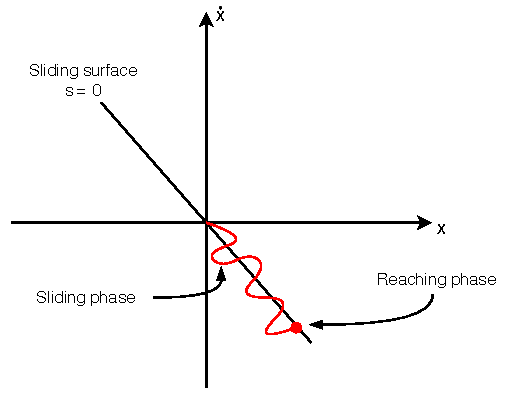
\includegraphics[width=0.5\linewidth]{figures/SM}
	\caption{Sliding mode behavior }
	\label{fig:SM}
\end{figure}

Introducing the small signal deviation of the states as
\begin{flalign}
	\vec{\tilde{q}} = \vec{  \bar{q}}^{-1} \otimes \vec{ q} 
	\label{eq:smallsignal22}
\end{flalign}
for the quaternion error and with $\vec{  \bar{q}}^{-1}$ be the reference quaternion and $\vec{ q} $ be the measured, and for the angular velocity
\begin{flalign}
	\vec{\tilde{\omega}}  = \vec{\omega}-\vec{\bar{\omega}}  
	\label{eq:smallsi4gnal4566}
\end{flalign}
with $\vec{\bar{\omega}}$ be the nominal value of the angular velocity. Moreover, by introducing the sliding variable as $s$ which depends on the error \nomenclature[S]{s}{Sliding variable} and is chosen to be 

\begin{flalign}
	s  = \underline{F}\vec{\tilde{q}} + \vec{\tilde{\omega}}  
	\label{eq:sliding variable}
\end{flalign}
with $\underline{F} = \alpha\ast diag[111]$ be a positive definite matrix. For $s=0$, $\vec{\tilde{\omega}} = - \alpha\ast\vec{\tilde{q}_{1:3}}$, where $\vec{\tilde{q}_{1:3}}$ denotes the vector part of the quaternion, and thus $\alpha$ can be designed appropriately, by trial and error to give the desired convergence for $\vec{\tilde{q}}$ meaning $[0;0;0;1]$, more details can be found in \todo{create appendix}.
The variable $s$ can be driven to 0 making use of a Lyapunov candidate function as
\begin{flalign}
	V  = \frac{1}{2} \vec{s}^{T}\vec{s} 
	\label{eq:sliding variable333}
\end{flalign} 
and in order to prove stability around $s=0$ a necessary condition is $\dot{V} < 0 $ for each $s\neq0$. The time derivative of \eqref{eq:sliding variable333} is written as
\begin{flalign}
	\dot{V}  = \frac{1}{2}( \dot{\vec{s}^{T}}\vec{s}+\vec{s}^{T}\dot{\vec{s}}) 
	\label{eq:sliding variable33333}
\end{flalign}
showing that $\vec{s}^{T}\dot{\vec{s}} < 0 $ $\forall s\neq0$ the condition may be satisfied.
Substituting \eqref{eq:sliding variable} is obtained
\begin{flalign}
	\dot{V}  = \vec{s}^{T} (\underline{F}{\vec{\dot{\tilde{q}}}} + {\vec{\dot{\tilde{\omega}}}}) 
	\label{eq:e33333}
\end{flalign}
and thus replacing \eqref{eq:seom} expressed for ${\vec{\dot{\tilde{\omega}}}}$ \eqref{eq:e33333} is written as 


\begin{flalign}
	\dot{V}  = \vec{s}^{T}\underline{I}_{s}^{-1}(-\underline{{\omega}}^\times\underline{I}_{s}\vec{\omega}-\underline{{\omega}}^\times\vec{h_{rw}}-\vec{N_{rw}}+\vec{N_{dis}} - \underline{I}_{s}\dot{\bar{\omega}} +\underline{I}_{s}\underline{F}{\vec{\dot{\tilde{q}}}} ) 
	\label{eq:444444}
\end{flalign}
by choosing the control as
\begin{flalign}
	\vec{N_{rw}}  = -\underline{{\omega}}^\times\underline{I}_{s}\vec{\omega}-\underline{{\omega}}^\times\vec{h_{rw}} - \underline{I}_{s}\dot{\omega} +\underline{I}_{s}\underline{F}{\vec{\dot{\tilde{q}}}}+\underline{I}_{s}\lambda sign(\vec{s})  ) 
	\label{eq:555555}
\end{flalign}

it can be seen in the above equations that the torque from the magnetorquers is not included since the magnetorquers are used only for desaturation.
\Eqref{eq:444444} can now be written as 
\begin{flalign}
	\dot{V} = -\vec{s}^{T}(-{\vec{\dot{\tilde{\omega}}}} +\lambda sign(\vec{s}) - \vec{N_{dis}}  )
	\label{eq:6666666}
\end{flalign}
consequently the condition $\dot{V} < 0 $ is satisfied if $\lambda >\rVert {\vec{\dot{\tilde{\omega}}}_{max}}\rVert +\rVert \vec{N_{dis}}\rVert$. The discontinuous function $sign$ is replace by the hyperbolic tangent function $tanh(\frac{\vec{s}}{\epsilon})$ in order to reduce the chattering around the manifold and $\epsilon$ is designed by trial and error.

